\documentclass[12pt]{../manual}
%____________________________________________________________________________
%
%	TITLE AND TABLE OF CONTENTS
%____________________________________________________________________________
\begin{document}
\makeheader{Lab 4}
\begin{center}
\textbf{\huge ECE 230L - LAB 4}\\~\\
\textbf{\large INTRODUCTION TO CIRCUIT SIMULATION USING PSPICE}\\~\\
\rule{6.5in}{0.5mm}
\end{center}

\tableofcontents

\listoffigures

\newpage
%____________________________________________________________________________
%
%	BODY
%____________________________________________________________________________
\section{Objectives of this Laboratory}
The objectives of this laboratory session are to introduce you to the basics of PSpice by learning:
\begin{itemize}
\item How to set-up your PSpice simulation environment,
\item How to represent the circuit elements,
\item How to construct the circuits, and
\item How to simulate the circuits.
\end{itemize}
%____________________________________________________________________________
%
% 	ORCAD
%____________________________________________________________________________
\section{Setting Up a Project Using ORCAD Capture}
To create a circuit in a PSpice environment, one must first launch ORCAD:
\begin{enumerate}
	\item Open Capture CIS 17.4
	\item Select Allegro PCB Librarian XL
	\item Create a new project by selecting {\bf File} $\to$ {\bf New} $\to$ {\bf Project}
	\item Name your project `Lab 4' and select the checkbox next to Enable PSpice Simulation
	\item Select {\bf Create a blank project} if prompted
\end{enumerate}

\begin{figure}[ht!]
	\begin{center}
		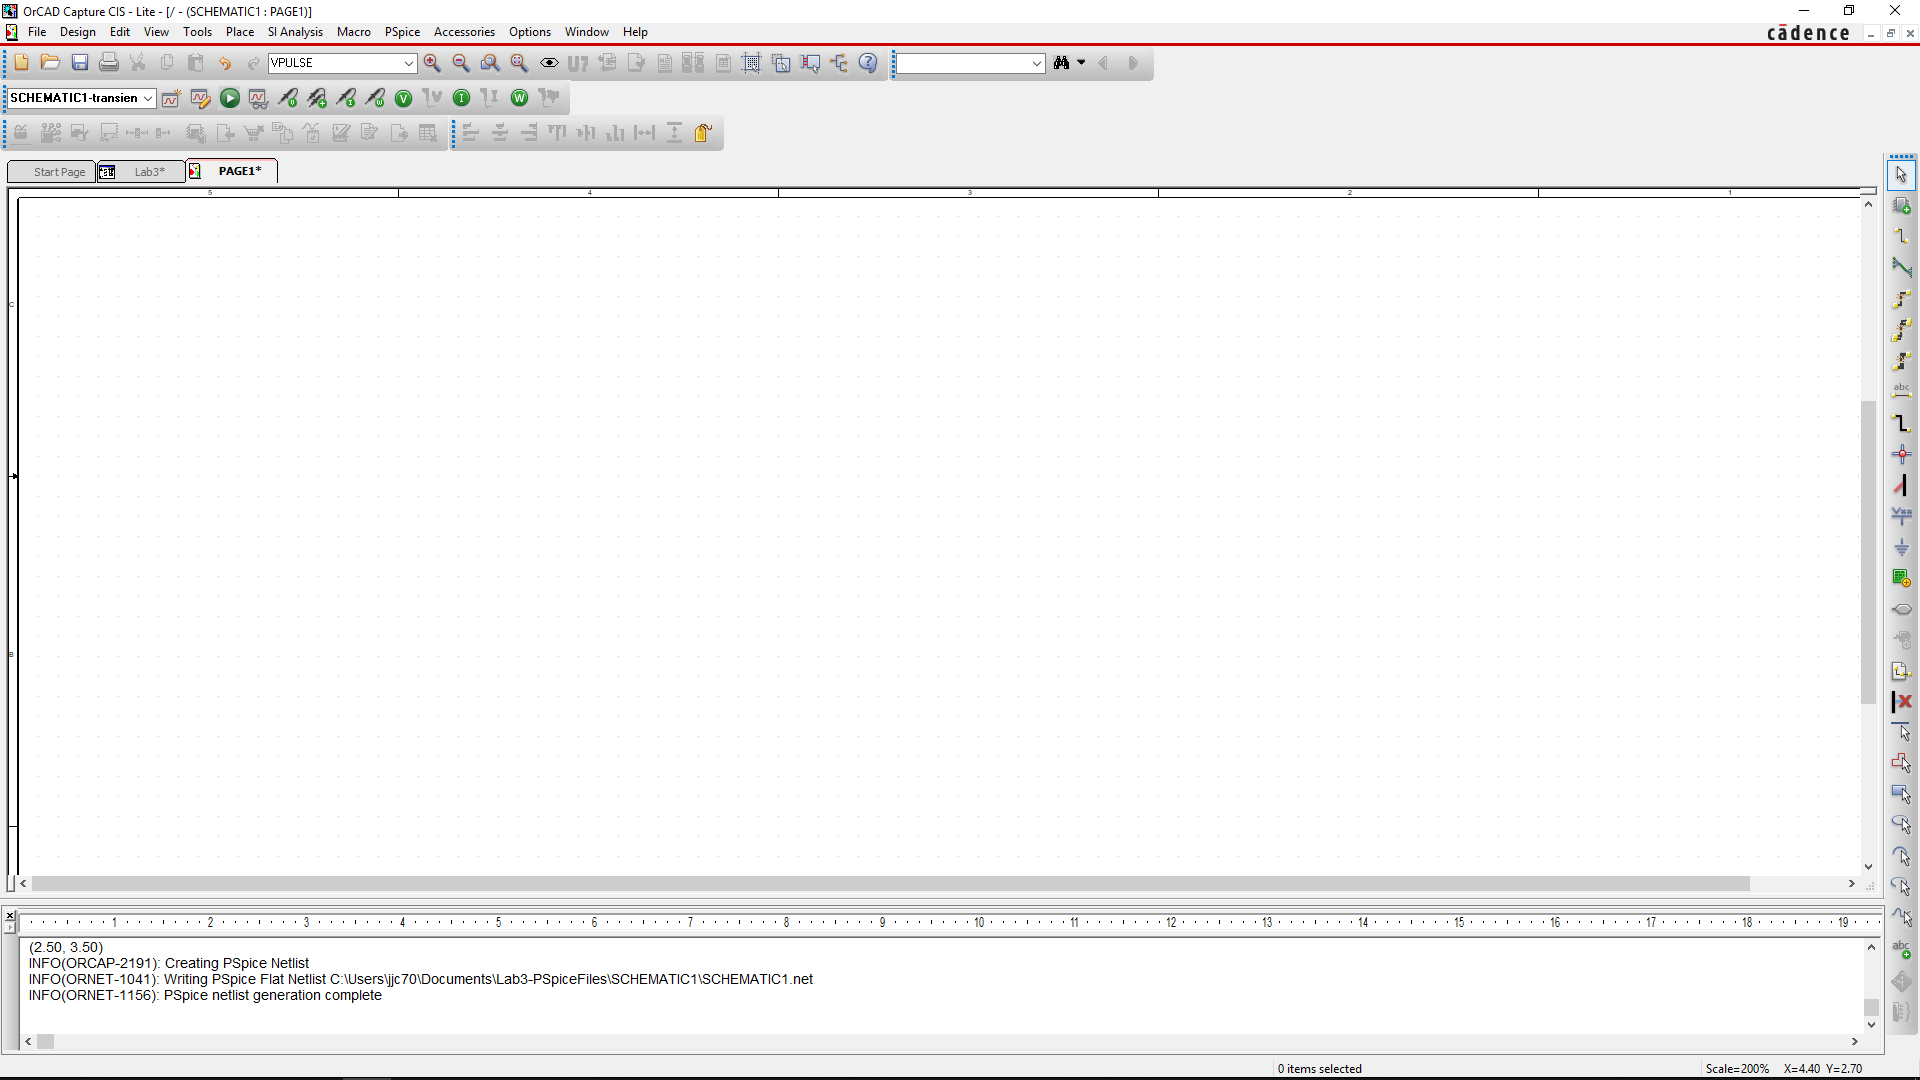
\includegraphics[width=0.9\textwidth]{./figures/BlankSchematic.PNG}
	\end{center}
	\caption{Blank Schematic}
	\label{fig:blankSchematic}
\end{figure}

Once the new project has been created, circuit design can begin. Sources, components, ground nodes, and wires can be selected using the {\bf Place} menu.

%____________________________________________________________________________
%
%	DC Analysis
%____________________________________________________________________________
\newpage
\section{DC Analysis in PSpice}

PSpice will be used to model and perform analyses on the circuit in Figure \ref{fig:dc}. To create the circuit, follow the steps below:
\begin{enumerate}
	\item Add a DC Voltage Source: \textbf{Place $\to$ PSPice Component $\to$ Source $\to$ Voltage Source $\to$ DC}
	\item Insert Resistors and Capacitors: \textbf{Place $\to$ PSpice Component $\to$ Passives} (Note that you can use Ctrl-R to rotate the components) 
	\item Insert Wires and connect circuit nodes: \textbf{Place $\to$ Wire}
	\item Insert a Ground: \textbf{Place $\to$ Ground $\to$ 0/SOURCE or 0/CAPSYM}
\end{enumerate}

\begin{figure}[ht!]
	\begin{center}
		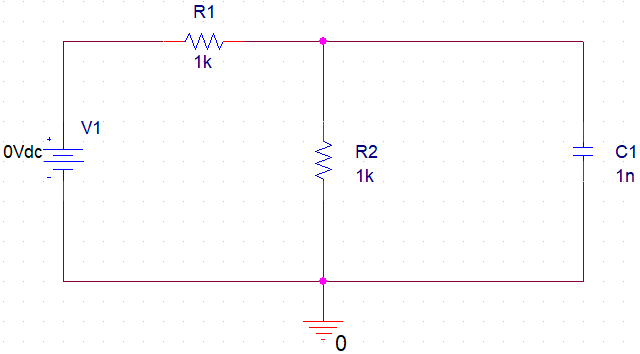
\includegraphics[width=0.9\textwidth]{figures/DCAnalysisCircuitCrop.PNG}
	\end{center}
	\caption{Circuit for DC Analysis}
	\label{fig:dc}
\end{figure}

To change values of any component, double click on the component and change the values using the pop-up menu. You may also change values by double clicking directly on the value and typing a new value.

To perform a DC analysis of the circuit, create a new simulation profile by selecting \textbf{PSpice} $\to$ \textbf{New Simulation Profile}. This may take a while to open. The bottom left of the window should say "Communicating with System...", this does not mean PSpice is frozen, just wait for it to finish loading. Name the new profile `dc' and press \textbf{Create}. Then,  select \textbf{DC Sweep} in the \textbf{Analysis Type} drop down menu, select \textbf{Primary Sweet} in the \textbf{Options}, and use the following parameters:
\begin{itemize}
\item Sweep variable $\to$ Voltage source: V1
\item Sweep Type: Linear
\item Start Value: 0
\item End Value: 10
\item Increment: 0.01
\end{itemize}

Press \textbf{Apply} and \textbf{OK} to save the profile settings. 

Begin the simulation by selecting \textbf{PSpice} $\to$ \textbf{Run}. This may also take a while to load. A new window should apear and the output window should say "Simulation running..." Again, just let the program finish. To view the circuit behavior at a particular point in time, follow \textbf{Trace} $\to$ \textbf{Add Trace} to select different values to plot. Plot V(R1:1) and V(R1:2) in one plot. Then, follow \textbf{Plot} $\to$ \textbf{Add Plot to Window} to create a new plot and add I(R1), and I(R2) to it. Figure \ref{fig:dcAnalRes} shows the result of DC analysis.

\begin{figure}[ht!]
\begin{center}
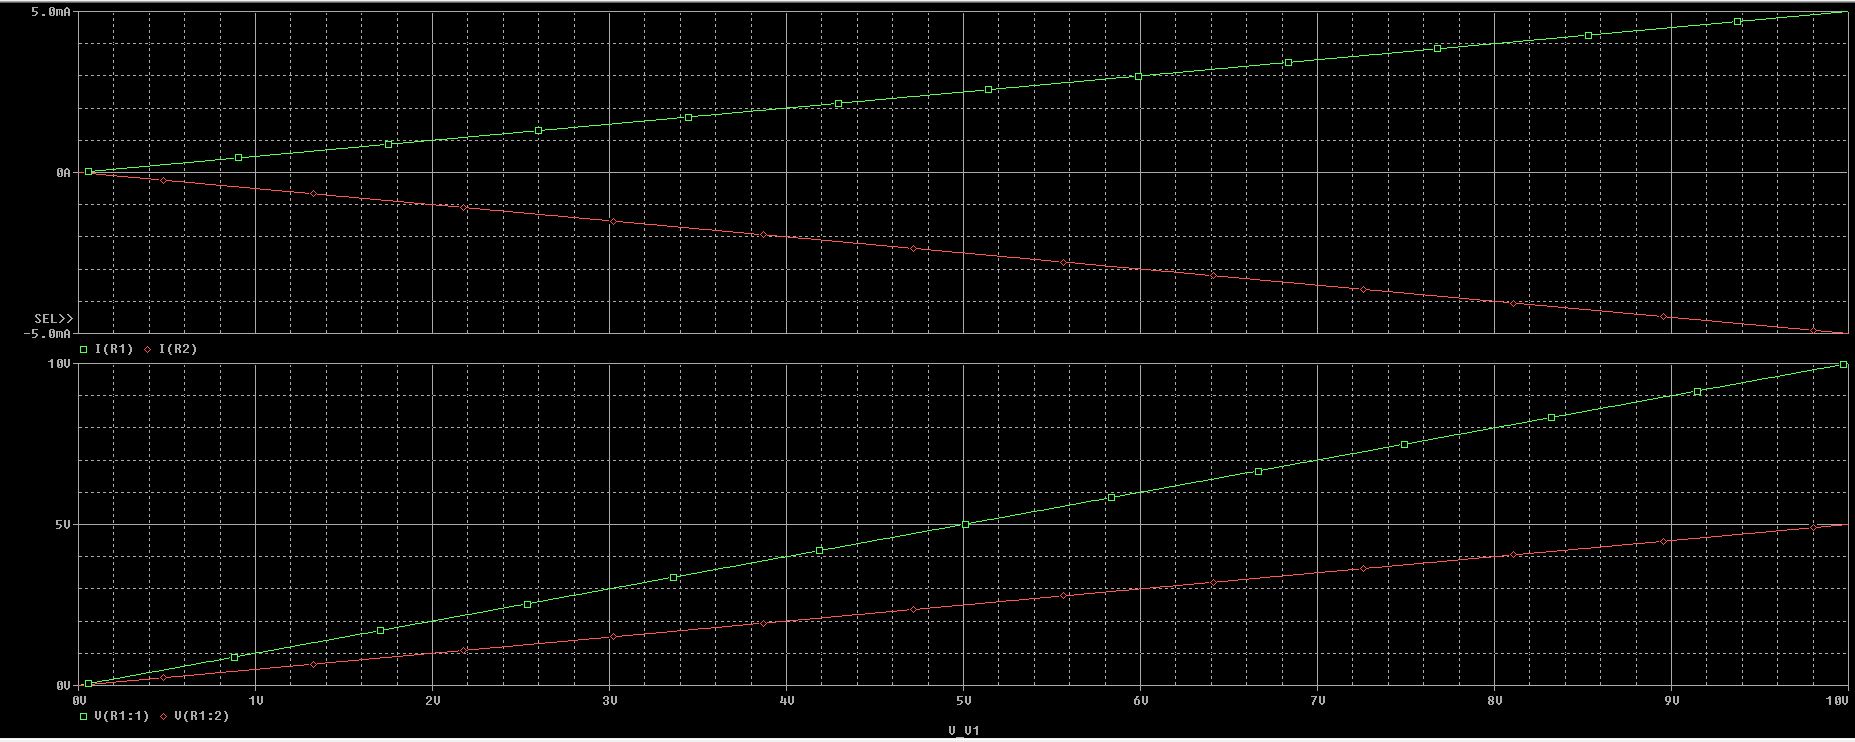
\includegraphics[width=\textwidth]{figures/ResultDCAnalysisCrop.PNG}
\caption[Result of DC Analysis]{Result of DC Analysis. Top: Current; Bottom: Voltage}
\label{fig:dcAnalRes}
\end{center}
\end{figure}
%____________________________________________________________________________
%
%	AC Analysis
%____________________________________________________________________________
\newpage
\section{AC Analysis in PSpice}
Before performing an AC analysis, a new AC voltage source has to replace the DC source. To change the source, delete the DC source and follow \textbf{Place} $\to$ \textbf{PSpice Component} $\to$ \textbf{Source} $\to$ \textbf{AC}. The following parameters will be used:
\begin{itemize}
\item DC Value: 10
\item AC Amplitude: 1
\end{itemize}

\begin{figure}[ht!]
	\begin{center}
		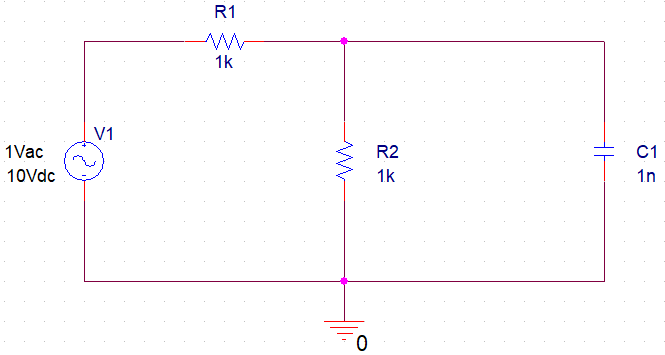
\includegraphics[width=0.9\textwidth]{figures/ACAnalysisCircuitCrop.PNG}
	\end{center}
	\caption{Circuit for AC Analysis}
	\label{fig:ac}
\end{figure}

After the voltage source properties have been changed, AC analysis can be performed. First, create a new simulation profile called `ac'. Next, select \textbf{AC Sweep/Noise} in the \textbf{Analysis Type} drop down menu and use the following parameters:
\begin{itemize}
\item AC Sweep Type: Logarithmic 
\item Select \textbf{Decade} from drop down menu below
\item Start Frequency: 1k
\item Stop Frequency: 1Meg
\item Number of Points per Decade: 10
\end{itemize}
Press \textbf{Apply} and \textbf{OK} to save the profile settings. They should look like Figure \ref{fig:acSettings}.

Now, begin the simulation by selecting \textbf{PSpice} $\to$ \textbf{Run}.

\subsection*{Trace Expressions in PSpice}
Trace expressions can be used to plot the phase of a desired value, a parameter in units of dB, or plot other useful mathematical operations on circuit parameters. Trace expressions are available under the \textbf{Trace} $\to$ \textbf{Add Trace} menu. Plot V(R1:2). Select \textbf{Plot} $\to$ \textbf{Add Plot to Window} and plot the value of V(R1:2) in dB by using the trace expression DB(V(R1:2)). Next, add another plot to the window and plot the phase of V(R1:2). Use the trace expression P(V(R1:2)). The resulting plots are shown in Figure \ref{fig:acAnalRes}.

\begin{figure}[ht!]
\begin{center}
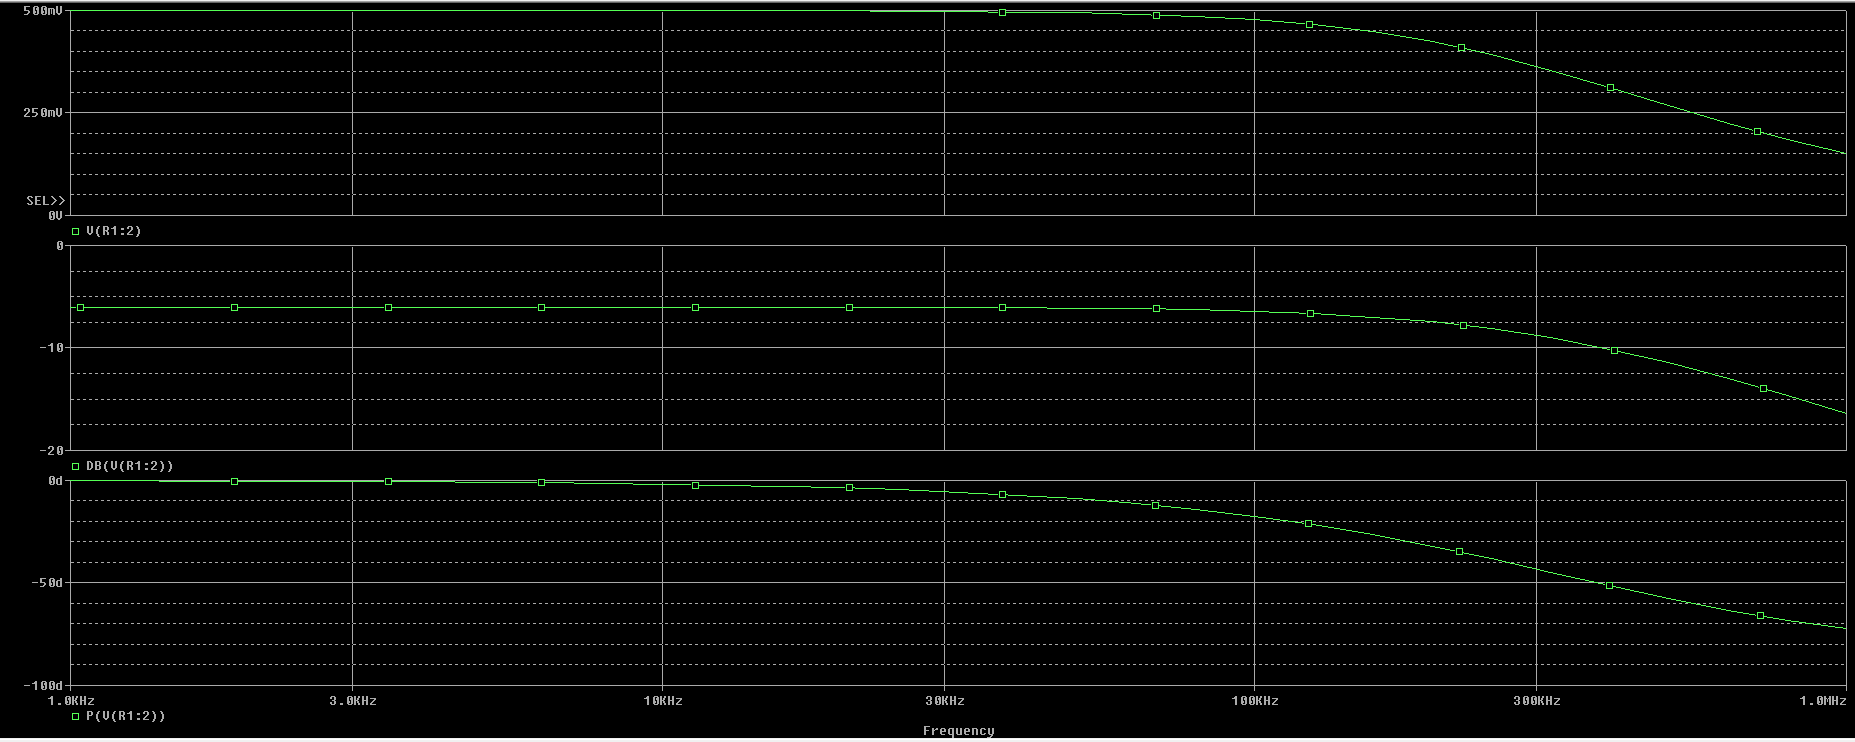
\includegraphics[width=\textwidth]{figures/ResultACAnalysisCrop.PNG}
\caption{Result of AC Analysis}
\label{fig:acAnalRes}
\end{center}
\end{figure}
%____________________________________________________________________________
%
%	Transient Analysis
%____________________________________________________________________________
\newpage
\section{Transient Analysis in PSpice}
Before performing a transient analysis, replace the AC source with a Pulse source (\textbf{Place} $\to$ \textbf{PSpice Component} $\to$ \textbf{Source} $\to$ \textbf{Pulse}). The following parameters will be used to set up the pulse: 
\begin{itemize}
\item V1 = 0
\item V2 = 5 
\item TD = 10n 
\item TR = 20n 
\item TF = 20n 
\item PW = 500n 
\item PER = 2u
\end{itemize}

We include the circuit in Figure \ref{fig:trans}.

\begin{figure}[ht!]
	\begin{center}
		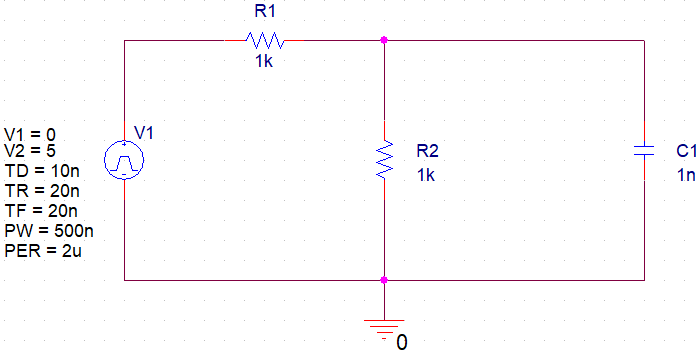
\includegraphics[width=0.9\textwidth]{figures/TransientAnalysisCircuitCrop.PNG}
	\end{center}
	\caption{Circuit for Transient Analysis}
	\label{fig:trans}
\end{figure}

After creating the circuit, create a new simulation profile called ``transient''. To analyze the new circuit, select \textbf{Time Domain (Transient)} in the \textbf{Analysis Type} drop down menu and use the following parameters:
\begin{itemize}
\item Run to Time: 2u
\item Start saving data after: 0
\item Maximum step size: 10n
\end{itemize}
Press \textbf{Apply} and \textbf{OK} to save the profile settings. 

Begin the simulation by selecting \textbf{PSpice} $\to$ \textbf{Run}. 

Plot the source voltage, V(R1:1), and V(R1:2). The resulting plot is shown in Figure \ref{fig:transAnalRes}.

\begin{figure}[ht!]
	\begin{center}
		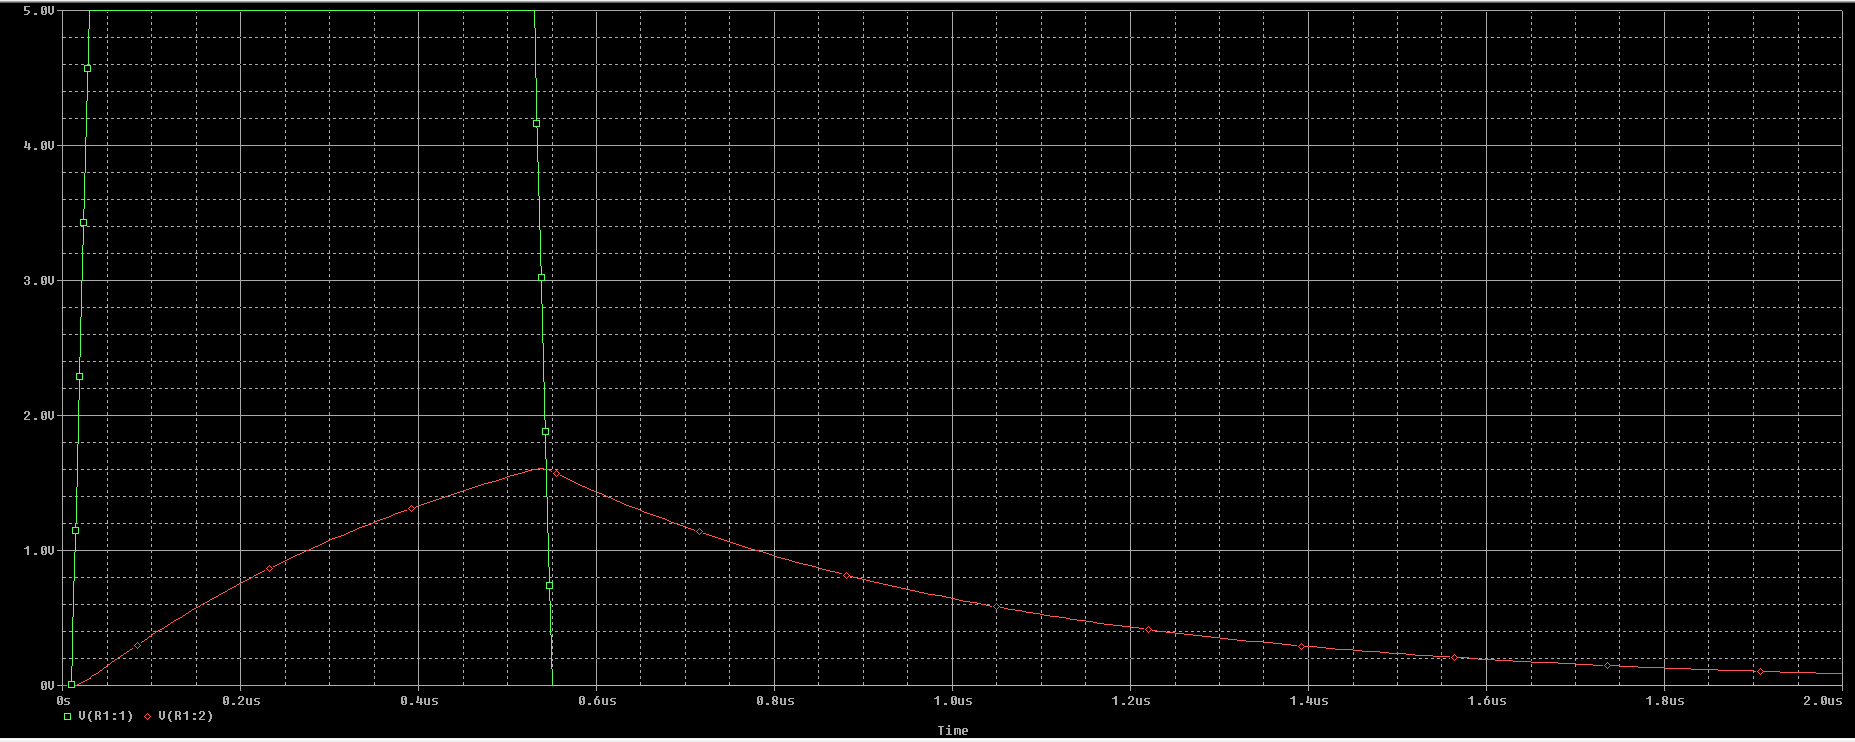
\includegraphics[width=\textwidth]{figures/ResultTransientAnalysisCrop.PNG}
	\end{center}
	\caption{Result of Transient Analysis}
	\label{fig:transAnalRes}
\end{figure}
%____________________________________________________________________________
%
%	Practice Example
%____________________________________________________________________________
\newpage
\section{Practice Example}
Use PSpice to simulate the circuit shown in Figure \ref{fig:practice} using DC, AC, and Transient analyses. Take a screencap of a plot of the voltage across capacitor $C_1$ in each analysis.

\begin{figure}[ht!]
\begin{center}
\begin{circuitikz}[scale=1.5]
%\ctikzset{resistors/scale=1.5,batteries/scale=1.5,grounds/scale=2.0,diodes/scale=1.5}
\draw
(0,0) 	to[short, *-] 	++(0,1)
		to[C, l=${C_1=\SI{1}{\nano\farad}}$]	++(2,0)
		to[short, -*]	++(0,-1)
		to[short]		++(1,0)
		to[R, l=${R_{sec}=\SI{1}{\kilo\ohm}}$] 	++(0,-2)
		to[short, -*]		++(-2,0)
		node[ground] {}
		to[short]		++(-2,0)
(2,0)	to[R, l=${R_{fir}=\SI{1}{\kilo\ohm}}$] 	++(-2,0)
		to [short] ++ (-1,0)
		to[battery, l_=${v_1}$, i=${i_{IN}}$] 	++(0,-2)
;\end{circuitikz}
\caption{Practice Circuit}
\label{fig:practice}
\end{center}
\end{figure}

\begin{enumerate}
\item In the DC analysis, use the following parameters:
\begin{itemize}
\item Sweep Type: Linear
\item Start Value: 0
\item End Value: 10
\item Increment: 0.01
\end{itemize}
\item In the AC analysis, change the voltage source to have the following values:
\begin{itemize}
\item DC Value: 5
\item AC Amplitude: 1
\end{itemize}
And use the following parameters:
\begin{itemize}
\item AC Sweep Type: Logarithmic 
\item Start Frequency: 10
\item Stop Frequency: 1Meg
\item Number of Points per Decade: 10
\end{itemize}
\newpage
\item In the transient analysis, change the voltage source to have the following values:
\begin{itemize}
\item V1 = 0, 
\item V2 = 5, 
\item TD = 100n, 
\item TR = 40n, 
\item TF = 40n, 
\item PW = 500n, 
\item PER = 2u
\end{itemize}
And use the following parameters:
\begin{itemize}
\item Run to Time: 2u
\item Start saving data after: 50n
\item Maximum step size: 10n
\end{itemize}
\end{enumerate}
%____________________________________________________________________________
%
%	Exploration
%____________________________________________________________________________
\newpage
\section{Exploration: Th\'evenin Equivalent Circuits}
\subsection*{Purpose}
The purpose of this exercise is to learn how to form a Th\'evenin Equivalent circuit by using circuit parameters obtained during simulation.

\subsection*{Introduction}
Any linear DC circuit as seen at a pair of terminals can be reduced to a practical voltage source (an ideal voltage source in series with a resistor).

\begin{figure}[ht!]
\begin{center}
\begin{circuitikz}[scale=1.5]
%\ctikzset{resistors/scale=1.5,batteries/scale=1.5,grounds/scale=2.0,diodes/scale=1.5}
\draw
(0,0)	to[R, *-, l=${R_{TH}}$]		++(-4,0)
		to[battery, l=${V_{OC}}$] 	++(0,-2)
		to[short, -*]	++(4,0)
(0,0.25)	node[] {A}
(0,-1.75)	node[] {B}
;\end{circuitikz}
\caption{Th\'evenin Equivalent Circuit}
\label{fig:thev}
\end{center}
\end{figure}

To form a Th\'evenin Equivalent circuit, two quantities must be calculated, measured, or simulated:
\begin{itemize}
\item $v_{oc}$: The open circuit voltage drop from terminals A to B
\item $i_{sc}$: The short circuit current from terminals A to B
\end{itemize}
Once the values for $v_{oc}$ and $i_{sc}$ have been obtained, the Th\'evenin resistance $R_{TH}$ can be determined using the relation:
\begin{align}
R_{TH} = \frac{v_{oc}}{i_{sc}} \label{eq:rth}
\end{align}
If the circuit contains no dependent sources, then $R_{TH}$ may also be found by turning off all of the independent sources and using resistance reduction at terminals A and B.

\newpage
\subsection{Example Exercise}
Simulate the circuit in Figure \ref{fig:exampleCircuit} and form its Th\'evenin Equivalent as seen from terminals A and B.

\begin{figure}[ht!]
\begin{center}
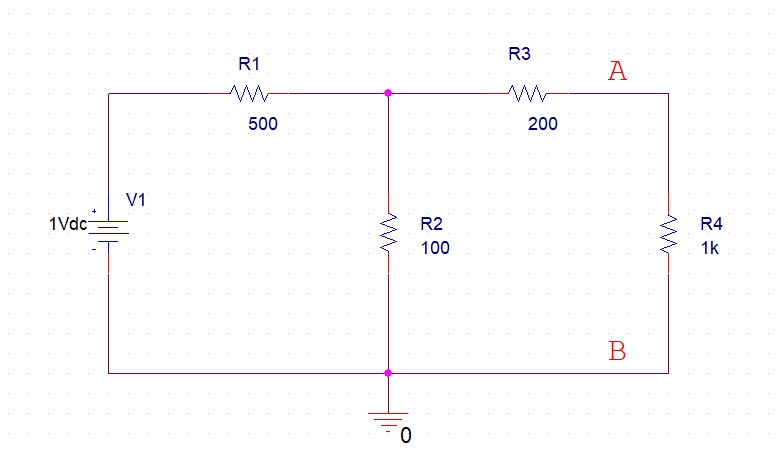
\includegraphics[width=0.7\textwidth]{figures/ExampleCircuitSchematicCrop.PNG}
\caption{Example Circuit}
\label{fig:exampleCircuit}
\end{center}
\end{figure}

To find the open circuit voltage, replace resistor $R_4$ with a large ``dummy'' resistance (at least \SI{100}{\mega\ohm}). Create a new simulation profile called ``thev''. Choose \textbf{Bias Point} under the \textbf{Analysis type} menu and check the box labeled \textbf{Include Detailed Bias Point Information} under the \textbf{Output File Options} heading. Press \textbf{Apply} and \textbf{OK} to save the profile. Now, run the simulation. Once the simulation is complete, follow \textbf{PSpice} $\to$ \textbf{Bias Points} and click \textbf{Enable}. Record the voltage across terminals A and B as your open circuit voltage.

\begin{figure}[ht!]
\begin{center}
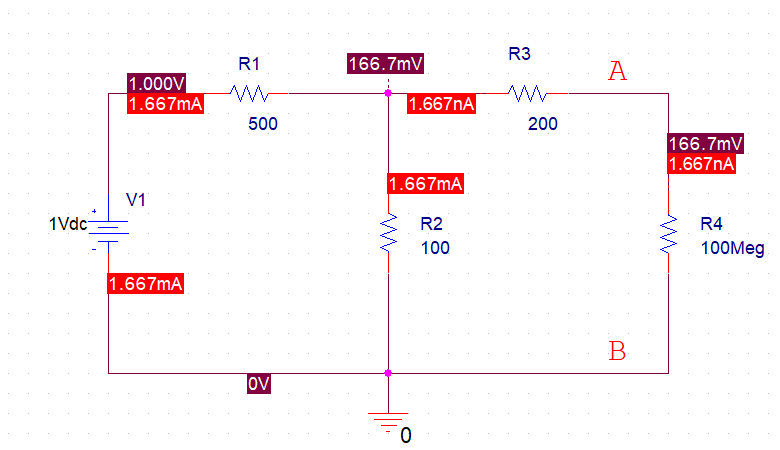
\includegraphics[width=0.7\textwidth]{figures/OpenCircuitSchematicCrop.PNG}
\caption{Open Circuit Voltage Schematic}
\label{fig:openCircuit}
\end{center}
\end{figure}

To find the short circuit current, remove $R_4$ and connect terminals A and B with a wire.
Use the same ``thev'' simulation profile that was created to find $v_{oc}$. Run the simulation. Once the simulation is complete, enable bias points. This will show the node voltages and currents throughout the circuit. Record the current between terminals A and B as your short circuit current, $i_{sc}$.

\begin{figure}[ht!]
\begin{center}
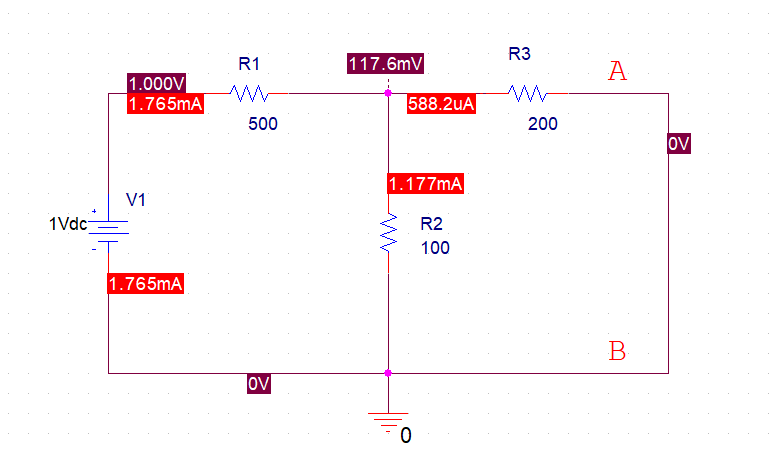
\includegraphics[width=0.7\textwidth]{figures/ShortCircuitSchematicCrop.PNG}
\caption{Short Circuit Voltage Schematic}
\label{fig:shortCircuit}
\end{center}
\end{figure}

Calculate the Th\'evenin resistance using Equation \ref{eq:rth}. Now, re-create Figure \ref{fig:thev} in PSpice using your $v_{oc}$ and $R_{TH}$ values. Place $R_4$ back into your first circuit and place a resistor of equal value between terminals A and B in your Th\'evenin Equivalent. Run the simulation using the same ``thev'' profile. Once the simulation is complete, enable bias points. Check to make sure the terminal voltages and currents match for both circuits.

\begin{figure}[ht!]
\begin{center}
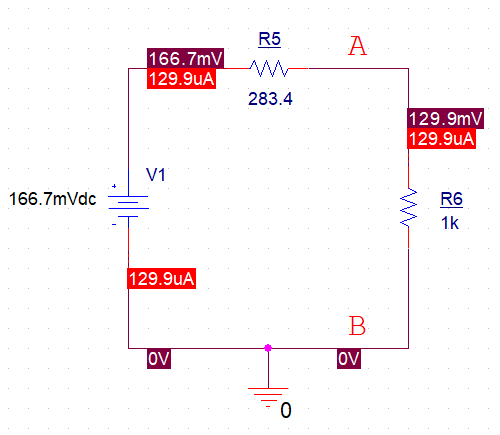
\includegraphics[width=0.5\textwidth]{figures/TheveninEquivalentExampleCrop.PNG}
\caption{Th\'evenin Equivalent Schematic}
\label{fig:thevCircuit}
\end{center}
\end{figure}

\newpage
\subsection{Challenge Exercise: Th\'evenin Equivalent Circuit}
Create the schematic in Figure \ref{fig:exerciseCircuit} using PSpice and find its Th\'evenin Equivalent circuit as seen from nodes A and B. In your lab report, be sure to include all voltages and currents present in the Exercise Circuit and its Th\'evenin Equivalent, as well as a short explanation of each step you took in finding the Th\'evenin Equivalent.
\begin{figure}[ht!]
\begin{center}
\begin{circuitikz}
%\ctikzset{grounds/scale=1.5}
\draw
(0,0) 	to[short] 		++(4,0)
		node[ground] {}
		to[short] 		++(4,0)
		to[R, l=$R_5$, a=\SI{500}{\ohm}]	++(0,4)
		to[R, l=$R_3$, a=\SI{200}{\ohm}]	++(0,4)
		to[short]		++(-8,0)
		to[battery, a=$V_1$, l=\SI{1}{\volt}]	++(0,-8)
(4,0)	to[R, *-, l=$R_2$, a=\SI{1}{\kilo\ohm}]			++(0,4)
		to[R, -*, l=$R_1$, a=\SI{100}{\ohm}]			++(0,4)
(4,4)	to[R, *-*, l=$R_4$, a=\SI{300}{\ohm}]			++(4,0)
(3.5,4) node[] {\textcolor{red}{A}}
(8.5,4) node[] {\textcolor{red}{B}}
;\end{circuitikz}
\caption{Exercise Circuit}
\label{fig:exerciseCircuit}
\end{center}
\end{figure}
%____________________________________________________________________________
%
%	Grading Rubric
%____________________________________________________________________________
\newpage
\phantomsection
\addcontentsline{toc}{section}{Grading Rubric}
\markboth{Grading Rubric}{Grading Rubric}
\hspace{0pt}
\vfill % used to center table vertically on page
\begin{table}[ht!]
\caption{ECE 230L Laboratory 4 Grading Rubric}
\centering
\begin{tabular}{l|c} \hline
Criteria & Points Possible \\ \hline \hline
\textbf{DC Analysis}			& \textbf{10} \\
Circuit Diagram 				& 5 \\
Waveforms 						& 5 \\ \hline
\textbf{AC Analysis}			& \textbf{10} \\
Circuit Diagram 				& 5 \\
Waveforms 						& 5 \\ \hline
\textbf{Transient Analysis}		& \textbf{10} \\
Circuit Diagram 				& 5 \\ 
Waveforms 						& 5 \\ \hline
\textbf{Practice Exercise}		& \textbf{35} \\
Circuit Diagram 				& 5 \\
DC Analysis						& 10 \\
AC Analysis						& 10 \\
Transient Analysis				& 10 \\ \hline
\textbf{Th\'evenin Equivalent Example Circuit} & \textbf{20} \\
Circuit Diagram					& 10 \\
$V_{OC}$ and $I_{SC}$ Labeled	& 5 \\
Correct $R_{TH}$ Value			& 5 \\ \hline
\textbf{Th\'evenin Equivalent Challenge Circuit} & \textbf{15} \\
Circuit Diagram					& 5 \\
$V_{OC}$ and $I_{SC}$ Labeled	& 5 \\
Correct $R_{TH}$ Value			& 5 \\ \hline \hline
\textbf{Total}					& \textbf{100} \\ \hline
\end{tabular}
\end{table}
\vfill % used to center table vertically on page
\end{document}
